\documentclass[12pt,letterpaper]{article}
\usepackage[utf8]{inputenc}
\usepackage[spanish, mexico]{babel}
\usepackage{amsmath}
\usepackage{amsfonts}
\usepackage{amssymb}
\usepackage{amsmath}
\usepackage[lmargin=3cm,rmargin=3cm,tmargin=3cm,bmargin=3cm]{geometry}

\usepackage{hyperref}
\usepackage{graphicx}
\usepackage{float}
\begin{document}

\title{Actividad 4: Ajuste de datos; ajuste de mínimos cuadrados}
\author{Luisa Fernanda Orci Fernandez.}
\date{15 de Febrero del 2016}

\maketitle

\section*{Ajuste de datos por mínimos cuadrados}
Mínimos cuadrados es una técnica de análisis numérico enmarcada dentro de la optimización matemática, en la que, dados un conjunto de pares ordenados: variable independiente, variable dependiente, y una familia de funciones, se intenta encontrar la función continua, dentro de dicha familia, que mejor se aproxime a los datos (un "mejor ajuste"), de acuerdo con el criterio de mínimo error cuadrático. En su forma más simple, intenta minimizar la suma de cuadrados de las diferencias en las ordenadas (llamadas residuos) entre los puntos generados por la función elegida y los correspondientes valores en los datos.  \cite{w}

\section{Optimize}
En esta actividad se nos proporcionó un código de la página Scipy Cookbook, en el cual se utiliza la función $optimize.leastsq$, de Scipy, también conocida como $optimize$. A través de datos podeos ajustar una curva a una función matemática. \\

El código proporcionado fue el siguiente:
\begin{verbatim}
import numpy as np
from numpy import pi, r_
import matplotlib.pyplot as plt
from scipy import optimize

# Generate data points with noise
num_points = 150
Tx = np.linspace(5., 8., num_points)
Ty = Tx

tX = 11.86*np.cos(2*pi/0.81*Tx-1.32) + 0.64*Tx+4*
((0.5-np.random.rand(num_points))*np.exp
(2*np.random.rand(num_points)**2))
tY = -32.14*np.cos(2*np.pi/0.8*Ty-1.94) + 0.15*Ty+7*
((0.5-np.random.rand(num_points))*np.exp
(2*np.random.rand(num_points)**2))
\end{verbatim}

\section{Actividad}
En esta actividad se nos solicitó hacer un ajuste líneal y otro exponencial por medio del método de mínimos cuadrados en Python. Para esto se nos proporcionaron dos listas de datos, una de ellas era la temperatura en invierno de la ciudad de Nueva York, la segunda era un registro de presión atmosférica vs altitud. Al de la temperatura es al que se le requiere hacer el ajuste líneal, y al de la presión el exponencial.

\subsection{Temperatura en invieron en Nueva York}
En base al código proporcionado, se elaboró uno nuevo para que este leyera el archivo y generara un ajuste líneal además de la gráfica.

\begin{verbatim}
import numpy as gatito
import matplotlib.pyplot as plt
from scipy.optimize import curve_fit

# Lee archivo de datos
data = gatito.loadtxt('tempdat.dat')

# Guarda las columnas en los vectores
x = data[:,0]
y = data[:,1]

# Ajuste lineal con parametros m,c
m, c = gatito.polyfit(x, y, 1)
xn = data[:,0]
# Evaluar xn en el ajuste calculado con los param m,c
yn = gatito.polyval([m, c], xn)

# Graficar datos y ajuste
plt.plot(data[:,0],data[:,1], 'ro')
plt.plot(xn, yn)

# Leyendas
plt.title("Temperatura de invierno en Nueva York en el siglo XX")
plt.xlabel("Fecha")
plt.ylabel("Temperatura promedio")
plt.legend(('data', 'fit'))
plt.grid(True)

plt.show()
\end{verbatim}
Nota: se tuvo que especificar que se leyera el archivo como dos columnas para lograr que lo graficara correctamente. La gráfica fue la siguiente:

\begin{center}
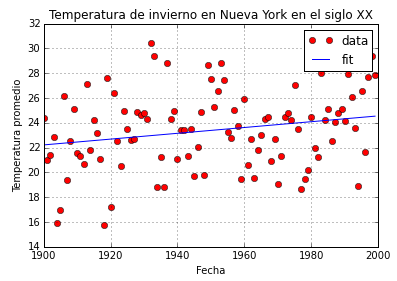
\includegraphics[scale=.7]{act4img2.png}
\end{center}

\subsection{Presión atmosférica vs Altitud}
Aquí se realizó un procedimiento similar al de la temperatura en la ciudad de Nueva York, pero esta vez con un ajuste exponencial y datos distintos. También se utilizó el arreglo para que se leyera la lista de datos en dos columnas.

\begin{verbatim}
import numpy as gatito
import matplotlib.pyplot as plt
from scipy.optimize import curve_fit

# Lee archivo de datos
data = gatito.loadtxt('presdat.dat')

# Guarda las columnas en los vectores
x = data[:,0]
y = data[:,1]
x = gatito.array(x, dtype=float) # convertir datos a reales
y = gatito.array(y, dtype=float) 

# Define funcion exponencial para interpolar los datos
def f(x, a, b, c):
    return c * np.exp(-a * x) + b

popt, pcov = curve_fit(f,x,y)

# Graficar datos y ajuste
plt.plot(data[:,0],data[:,1], 'ro')
plt.plot(x, y)

# Leyendas
plt.title("Presion atmosferica como funcion de la altura")
plt.xlabel("Altitud (km)")
plt.ylabel("Presion atmosferica (mb)")
plt.legend(('data', 'fit'))
plt.grid(True)

plt.show()
\end{verbatim}

La gráfica final fue la siguiente:

\begin{center}
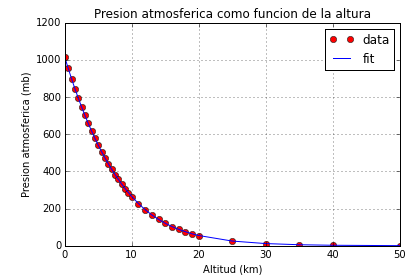
\includegraphics[scale=.7]{act4img1.png}
\end{center}

\section*{Conclusiones}
Esta actividad, así como las anteriores, es muy importnte, ya que pudimos aprener como utilizar esta herramienta computacional para en un futuro hacer ajustes de una forma mas sencilla y rápida en vez de hacerla a mano (lo digo como veterana del curso de Análisis Numérico), ya que el semestre pasado tuvimos que realizar ajustes y aproximaciones a mano y resultó ser muy tedioso.

\begin{thebibliography}{widestlabel}
\bibitem{w} $https://es.wikipedia.org/wiki/Minimos_-$cuadrados
\end{thebibliography}


\end{document}
